\documentclass[a4paper,12pt]{article}

\usepackage{amssymb}
\usepackage{amsmath}
\usepackage{amsfonts}
\usepackage{txfonts}
%\usepackage{upgreek}
\usepackage{graphicx}
%\usepackage{siunitx}
\usepackage{enumerate}
\usepackage[left=2cm,right=2cm,top=2cm,bottom=2cm]{geometry}

%\newcommand{\question}[2]{\textbf{\textit{#1}}\quad{\footnotesize\textit{(#2 points)}}\\[3mm]}
\newcommand{\question}[1]{\textbf{\textit{#1}}}
\newcommand{\points}[1]{\quad{\footnotesize\textit{(#1 points)}}}
\newcommand{\point}{\quad{\footnotesize\textit{(1 point)}}}
\newcommand{\HRule}{\rule{\linewidth}{0.3mm}}
\newcommand{\dd}{\mathrm{d}}
%\renewcommand{\pi}{\uppi}
\newcommand{\ii}{\mathrm{i}}
\renewcommand{\thefootnote}{\normalsize\fnsymbol{footnote}}
\DeclareMathOperator{\e}{e}
\newcommand{\bra}{\langle}
\newcommand{\ket}{\rangle}

\renewcommand{\theequation}{\Roman{equation}}

\begin{document}
\pagestyle{empty}

\begin{center}
\LARGE \textbf{Astronomy from 4 perspectives: the Dark Universe}
\HRule
\end{center}
\begin{flushright}
prepared by: Heidelberg participants and BMS
\end{flushright}
\begin{center}
{\Large \textbf{Tutorial: the Planet of the Petit Prince}}
\end{center}
\vspace{5mm}
{\bf Scope of the tutorial}
The scope of this tutorial is to create a set of exercises on
gravity, and basic mechanics, using as a reference the ``Planet of the
Petit Prince'' by A. de Saint-Exupery, in order to have students
familiarize with the basic scaling of gravitational forces, in a
set-environment different from Earth. This should help student
understand how to generalize and extrapolate the knowledge they have
gotten in school to problems that are unfamiliar. The first set of
exercises requires only basic knowledge of claassical mechanics (work,
and escape velocity) and the inverse square-distance law of
gravity. The second set of exercizes, more advanced, requires the
knowledge of the pendulum law and or Archimesdes principle. The third
set of exercises focus on the inhomogeneity of the graviational field,
and requires some basic knowledge of tidal forces and basic
relativity.

\begin{figure}[h]
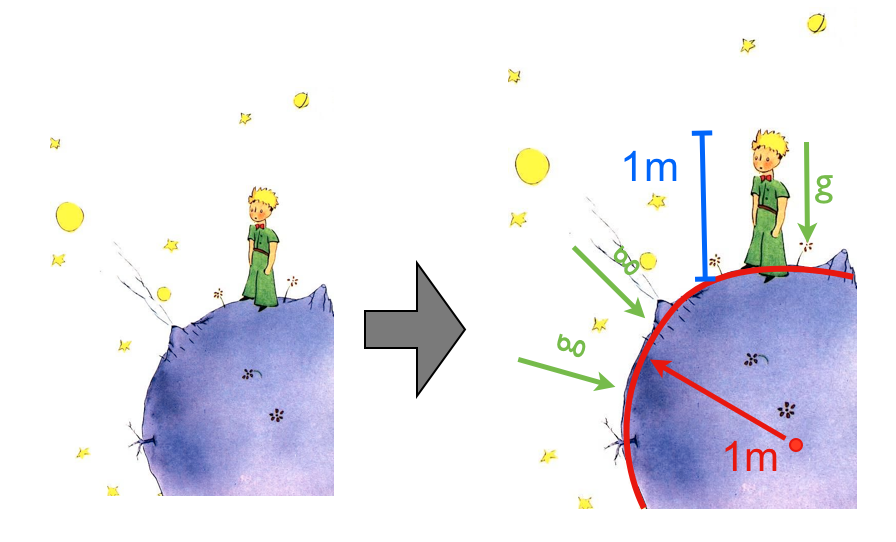
\includegraphics[width=16cm]{figure.png}
\caption{The planet of the petit price and its physical setup}
\end{figure}

{\bf Exercises}
\\
\begin{enumerate}[\itshape \bfseries 1.]

\item \question{Gravity on the planet of the Petit prince}\\
The Petit Prince by A. de Saint-Exupery lives on a planet which,
according to images, is roughly $R\simeq 1~\mathrm{m}$ in size and
because Saint-Exupery does not provide any other information, has a
value of the surface gravity $g=9.81~\mathrm{m}/\mathrm{s}^2$ similar
to Earth. But in comparison to Earth where the gradient of the
acceleration is almost zero, it is much stronger on the planet of the
Petit Prince. Recall that $G=6.6\times 10^{-11}$ in SI.
\begin{enumerate}[(a)]
\item{What is the density $\rho$ and mass $M$ of the planet, assuming that it is uniform? What astrophysical objects would have similar densities?}
\item{What would be the orbital velocity $\upsilon$ of an object at a height of $1~\mathrm{m}$ above the surface? Could the Petit Prince throw an object horizontally and have it orbit his planet?}
\item{Can the Petit Prince leave the planet by jumping into space?}
%\item{What is the pressure inside the planet? Can you estimate the pressure from the observation that the volcanic plume of one of the three volcanoes is about the same height as the Petit Prince?}
\item{Is it possible that the Petit Prince can observe 43 sunsets each day despite the centrifugal force? How many sunsets can one observe at most?}
\end{enumerate}

\item \question{devices on the planet of the Petit prince}\\
Imagine that Saint-Exupery brings simple mechanical systems with him, and find out if they behave differently because of the strong gradient $\partial g/\partial r$ in the gravitational acceleration $g$.
\begin{enumerate}[(a)]
\item{What's the relation between the oscillation period $T$ of a pendulum clock as a function of height $h$? Would the oscillation period be independent from the amplitude?}
\item{Saint-Exupery and the Petit Prince have a glass of orange juice
    with an ice cube. The Petit Prince's ice cube swims higher or not above the surface of the juice compared to Saint-Exupery's?}
\end{enumerate}

\item \question{relativity on the planet of the Petit prince}\\
Are there relativistic effects of gravity on the planet of the Petit Prince?
\begin{enumerate}[(a)]
\item{What is the tidal gravitational acceleration between the head
    and the feet of the Petit Prince? Please compute the difference
\begin{equation}
\Delta g = \frac{GM}{R^2}-\frac{GM}{(R+1)^2} 
\end{equation}
}
\item{What is the gravitational time dilation between the head and the feet of the Petit Prince? Please use the formula
\begin{equation}
\Delta \tau = \sqrt{1+2\frac{\Phi}{c^2}}\:\Delta t
\end{equation}
and approximate the potential as homogeneous, $\Phi = g\Delta r$.
}
\end{enumerate}
\end{enumerate}
\newpage

{\bf Solutions}
\\

\begin{enumerate}[\itshape \bfseries 1.]

\item \question{Gravity on the planet of the Petit prince}\\
The Petit Prince by A. de Saint-Exupery lives on a planet which,
according to images, is roughly $R\simeq 1~\mathrm{m}$ in size and
because Saint-Exupery does not provide any other information, has a
value of the surface gravity $g=9.81~\mathrm{m}/\mathrm{s}^2$ similar
to Earth. But in comparison to Earth where the gradient of the
acceleration is almost zero, it is much stronger on the planet of the
Petit Prince. Recall that $G=6.6\times 10^{-11}$ in SI.
\begin{enumerate}[(a)]
\item{The relation between the mass $M$and the density $\rho$ of the planet is
    $M=(4\pi /3)\rho R^3$. The surface gravity is tied to the mass by
    $g=GM/R^2$. Substituting one in the other, one can solve to find a
    density $\rho \simeq 3.5\times 10^{10}$ kg m$^{-3}$. This is quite
  close to the density of a White Dwarf.}
\item{The orbital period and velocity can be obtained by equation the
    gravitational acceleration to the centrifugal acceleration:
    $GM/(R+1\mathrm{m})^2 = \Omega^2 (R+1\mathrm{m}) $. This gives
    $\Omega \simeq 1$ s$^{-1}$ corresponding to a period $P\simeq 6$ sec, and
    an orbital speed $V=\Omega (R+1\mathrm{m})\simeq 4$ m
    s$^{-1}$. Yes the Petit Prince can throw an object fast enough to
    put it into orbital motion.}
\item{The escape speed is given by equating the specific kinetic
    energy $V^2/2$ to the potential energy $GM/R$, and this gives a
    typical value $V\simeq 4$ m
    s$^{-1}$. This is too much for a kid to jump.}
\item{Given that the maximum period is 6 sec (computed above, and our
    day corresponds to $86400$ sec then
    there will be at most $14000$ sunsets/sunrises.}
\end{enumerate}

\item \question{Devices on the planet of the Petit prince}\\
Imagine that Saint-Exupery brings simple mechanical systems with him, and find out if they behave differently because of the strong gradient $\partial g/\partial r$ in the gravitational acceleration $g$.
\begin{enumerate}[(a)]
\item{For small oscillations the formula for the oscillation period of
  a pendulum is $T=2\pi\sqrt{L/g}$ where $L$ is the length of the
  pendulum and $g$ is the gravitational acceleration. On this planet,
  at an heigh $h$ above the surface it will be:
  $g=GM/(R+h)^2$. Then $T=2\pi (R+h)\sqrt{L/GM}$. The period increases
  proportionally to the height. Given that $g$ is not constan with
  height, as the pendulum oscillates it will experience different
  acceleration (stronger at the bottom point, weaker at the edge points
  of its oscillating trajectory) so the pendulum formula does not
  apply, and there will be a dependence on the oscillation
  amplitude. One can try to use a mean values for $g$. Using some
  basic trigonomentry (see Figure 2) the difference in heigth between the bottom
  point and the edge point is $L(1-\cos{\theta})$, where $\theta$ is
  the amplitude of the oscillation. So the average $g \simeq
  GM/R^2[1+L(1-\cos{\theta})]/2R$. substituting this in the equation
  for the pendulum period $T$ one gets an estimate on how it depends
  on the apmplitude $\theta$.}
\item{Archimedes principle says that a body immersed in a liquid
    (water in our case) received a lift upward with a force equal to
    the weight of the volume of the liquid it displaces. With
    reference to the figure, let us consider an icecube of an edge of
    length $L$, floating in water with a depth equal to $h$ (see
    Figure 2). Let us
    call $\rho_{\rm I}$ the density of ice and $\rho_{\rm W}$ the
    density of wager. We know that ice is lighter than water, such
    that the former flots on latter. For conveneince we assume that
    the icecube is small enough that the gravity can be taken as
    uniform over its size. A typical icecube is $\sim 1$cm, while on
    the Petit Price planet the typical scale for the variation of
    gravity is $\sim 1$m. The gravitatinal force acting on
    the icecube is equal to $F_g=g\rho_{\rm I}L^3$. Archimedes force
  is instead $F_a=g\rho_{\rm W} h L^2$. The cube will float if the two
are equal, and this gives $h= L\rho_{\rm I}/\rho_{\rm W}$, that as one
can see does not depend on the graviational acceleration. So it does
not matter if the graviational field is stronger or weaker. The
icecube of the prince will float as much as the one of Saint Exupery.}


\begin{figure}[h]
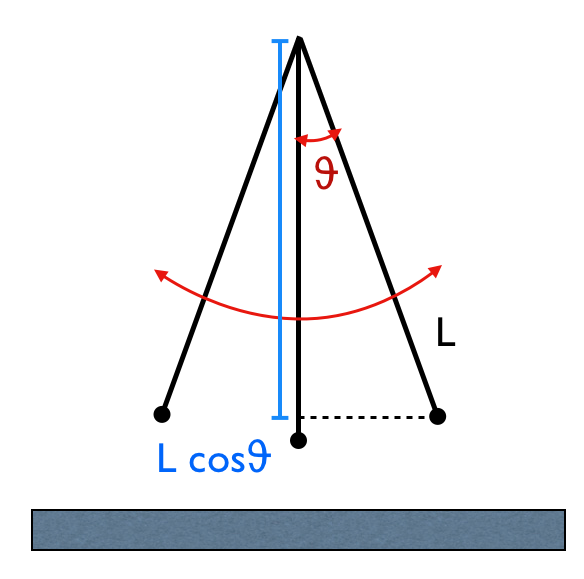
\includegraphics[width=8cm]{pendulum.png}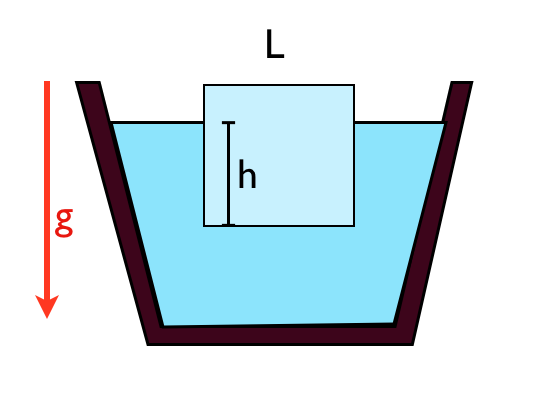
\includegraphics[width=8cm]{icecube.png}
\caption{Left: the geometry of a pendulum. Right: a floating icecube. }
\end{figure}

\end{enumerate}

\item \question{relativity on the planet of the Petit prince}\\
Are there relativistic effects of gravity on the planet of the Petit Prince?
\begin{enumerate}[(a)]
\item{What is the tidal gravitational acceleration between the head
    and the feet of the Petit Prince? Please compute the difference
\begin{equation}
\Delta g = \frac{GM}{R^2}-\frac{GM}{(R+1)^2} 
\end{equation}
}
\item{What is the gravitational time dilation between the head and the feet of the Petit Prince? Please use the formula
\begin{equation}
\Delta \tau = \sqrt{1+2\frac{\Phi}{c^2}}\:\Delta t
\end{equation}
and approximate the potential as homogeneous, $\Phi = g\Delta r$.
}
\end{enumerate}
\end{enumerate}

\end{document}
